\subsection{Classification by Templates Based on the Spectral Shape}
\label{section:method2}

The second method is based on the comparison of the spectral shape of the different stroke types. Therefore, in the training phase, templates for each trained drum and cymbal are created. These templates are used for comparison when classifying a stroke.

%a)create mean spectrum and use correlation coefficient for spectral shape comparison
%Dann brauchen wir ein Maß, das angibt, ob das Spektrum A und B
%übereinstimmt, wobei die Gesamtstärke keine Rolle spielen soll, nur die
%Form (spectral shape).  Dafür schlage ich vor:
%
  %sum (A .* B) / sqrt (sum (A.^2) * sum (B.^2)).
%
%Das ist aus der Statistik bekannt als (nicht zentraler)
%"Korrelationskoeffizient". Er ist 1, wenn A und B die gleiche Form
%haben, sonst kleiner und minimal -1.

%Sometimes, the exact relationship is not of interest, only the degree of association between two variables.
%This relationship (=association) is called the correlation between x and y. The strength of the correlation and whether it is negative or positive is given by a single statistic, r, the CORRELATION COEFFICIENT (also known as the Pearson Product Moment Correlation Coefficient):
%It is the ratio of the COVARIATION between x and y (corrected for their respective means) to the total variation in both x and y (once again corrected for their respective means)
%Covariation means just what the term implies - when (x - x-bar) is large (in absolute terms) and negative, is (y - y-bar) also large and negative? When x - x-bar is small and positive, is y - y-bar also small and positive?
%If (x - x-bar) is positive, and (y - y-bar) is positive, then the resulting term is positive
%If(x - x-bar) is negative, and (y - y-bar) is negative, then the resulting term is positive
%If (x - x-bar) is positive, and (y - y-bar) is negative, then the resulting term is negative
%If (x - x-bar) is negative, and (y - y-bar) is positive, then the resulting term is negative
%So you can see, that if x and y always match signs, the numerator will turn out to be positive, If they don't match, the numerator will be negative.
%The denominator is always positive due to the squaring, so whether or not r is positive or negative depends on the degree of matching in the numerator.
%A negative r indicates an inverse relationship (as x gets large, y gets large)
%r = 0 indicates no relationship between x and y
%A negative r indicates an inverse relationship (as x gets large, y gets small)

%Der empirische Korrelationskoeffizient als Maßzahl für die Stärke eines linearen Zusammenhangs wird mittels einer Normierung der empirischen Kovarianz durch das Produkt der Standardabweichung berechnet

The first approach to the comparison of the spectral shape was to use a correlation coefficient to compare the test instance $T$ with the training data. Therefore, a mean frequency spectrum $M$ from all training records for one class label is calculated. After that, the correlation coefficient is calculated from the vectors $T$ and $M$. The correlation coefficient $r$ is calculated by:

\begin{equation}
\label{eq:correlationcoefficient}
	r = \frac{\sum_{i=1}^{n}{(T_i * M_i)}}{\sqrt{\sum_{i=1}^{n}{(T_i^2)}\sum_{i=1}^{n}{(M_i^2)}}}
\end{equation}

%To test the correlation coefficient with MatLab\textsuperscript{\textregistered}, the following code was used:
%\lstinline{ r = sum (T .* M) / sqrt (sum (T.^2) * sum (M.^2)).}

This formula calculates the linear correlation in the spectral shapes of the two vectors $T$ and $M$ as a value between -1 and +1. If $T$ and $M$ represent the same drum or cymbal, the calculation shall return a value near one. The smaller the returned value, the smaller the correlation, the smaller the probability that the two spectra represent the same class label. Further information on correlation coefficients can be found in \autocite{Hedderich:2012}. 

%The empiric correlation coefficient $r_{xy}$ is described in \autocite{Hedderich:2012} as a measurement for the degree of the linear correlation between the variables $x_i$ and $y_i$. Like shown in the following formula (\ref{eq:correlationcoefficient}), it is calculated by the empiric covariance ($S_{xy}$) divided by the product of the standard deviations of $x_i$ and $y_i$ ($S_{x}S_{y}$). 
%
%\begin{equation}
%\label{eq:correlationcoefficient}
	%r_{xy} = \frac{S_{xy}}{S_x S_y} = \frac{\sum_{i=1}^{n}{(x_i-\bar{x})(y_i-\bar{y})}}{\sqrt{\sum_{i=1}^{n}{(x_i-\bar{x})^2}\sum_{i=1}^{n}{(y_i-\bar{y})^2}}}
%\end{equation}
%
%This formula returns a value $r$ between -1 and +1. A positive $r$ indicates a relationship between $x$ and $y$, a positive $r$ an inverse relationship. If $r = 0$, there is no relationship between $x$ and $y$. 

The use of the correlation between $T$ and $M$ leads to a low hit-rate, especially because of the varying amplitudes in a cymbal stroke. Here, the spectral shape differs a lot from stroke to stroke and also in the development of a single stroke. Thus, the correlation coefficient can be very small despite two equal drums are compared. This problem leads to a new approach that does not compare the test instance with the mean of the training data, but rather examines if the frequency bins of the test instance are located within an acceptable range. As displayed in figure \ref{fig:templates1}, this range is defined by two templates containing vectors. One defines the minimum and one the maximum limit for each bin in the drum strokes frequency spectrum. With this method a hit-rate of 97,2 \% is reached.

\begin{figure}[htb]
	\centering
	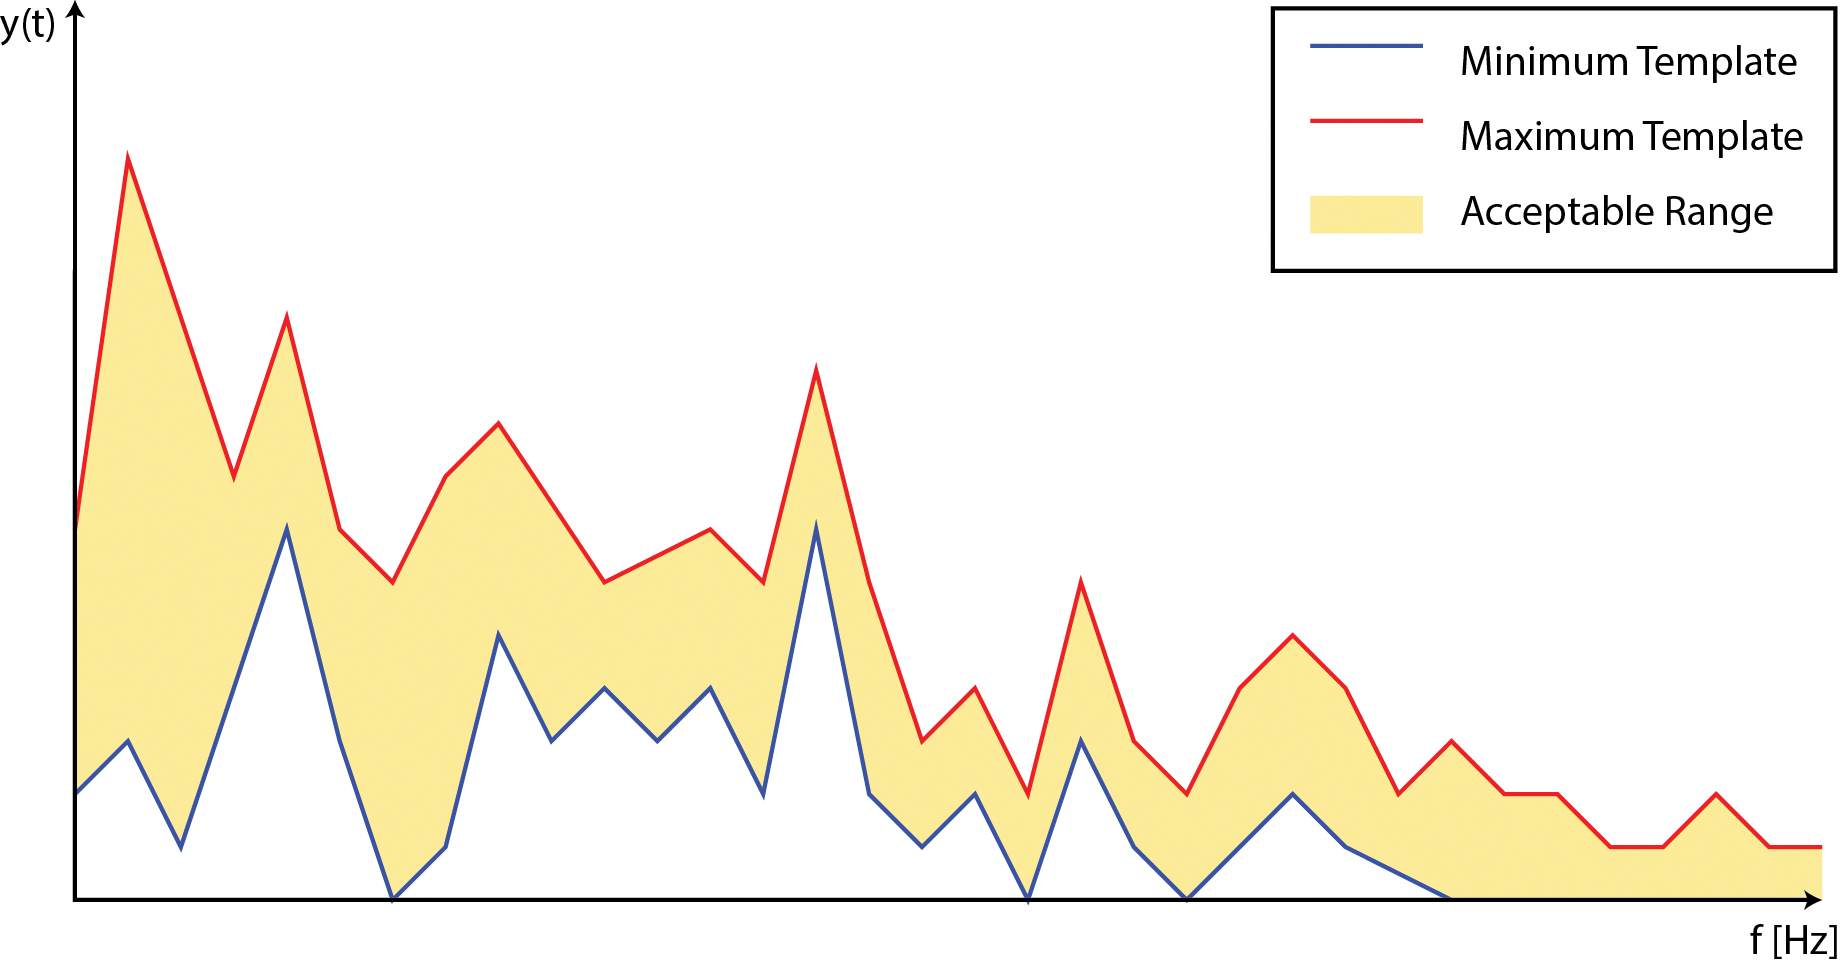
\includegraphics[height=5cm]{images/acceptable_range.png}
	\caption{Minimum and maximum template.}
	\label{fig:templates1}
\end{figure}

%If the resulting spectra of minimum and maximum amplitudes for a drum type are displayed, it can be seen, that the distance between the minimum and maximum bin at the most main peak positions is much smaller than the distance at non peak positioned bins. This leads to a smaller acceptable range in the classification step. The phenomena can be seen in figure \ref{fig:minmax}. It can be attributed to the fact that the main peaks of a stroke are more stable than other appearing frequencies, like shown in section \ref{section:classificationSpectrumAnalysis}. Because the main peaks can vary strong from stroke to stroke, the smaller acceptable range could cause errors in the classification step. This leads to the idea to create an additional template which only considers the peak positions within the frequency spectra of a record.

The creation of the templates is described in the following section. After that, three different methods for classification are tested. The methods are explained in sections \ref{section:shapeComparisonClassification1}, \ref{section:shapeComparisonClassification2} and \ref{section:shapeComparisonClassification3}.


\subsubsection{Template Creation} \label{section:shapeComparisonTemplates}

For the template creation the training data recorded as described in section \ref{section:training} is used. There are 24 different frequency spectra saved for each drum type. To use this frequency spectra for templating, each data record is pre-processed by onset detection, Fourier transform, noise reduction and normalization. Onset detection and Fourier transform are performed identically to the first classification method, which is described in section \ref{section:method1pre-processing}. For noise reduction and normalization an improved approach is used.

The new method for the noise reduction is developed in consideration of the usage in the final system. A future user might use a noisy microphone that interferes the drum sound, so it must be possible to filter every kind of noise. To realize that, an additional audio sequence containing silence is recorded. Thus, only the noise that is produced by the microphone is recorded. A frequency spectrum $N$ of the noise file is prepared for noise reduction as follows:

\begin{enumerate}
  \item The audio sequence $Y$ of the recorded file is loaded.
  \item The mean $M$ of three subsequent frames $Y_1, Y_2, Y_3$ extracted from the audio sequence is calculated, beginning with the first sample of the audio wave. Thereby, the frame size is 2048 samples, equal to the frame size used for the training set in section \ref{section:training}. The mean M is calculated by $(Y_1+Y_2+Y_3)/3$.
  \item The calculated mean $M$ is Fourier transformed to its frequency spectrum $N$ by MatLab\textsuperscript{\textregistered}s build in FFT function.
	\item The values of each amplitude bin $n_i$ in the frequency spectrum $N$ are transformed to its absolute values.
\end{enumerate}

%code
%[y_noise,fs] = audioread('silence.wav');
%noise = abs(fft(windowFunction.*((y(1:2048)+y(2049:4096)+y(4097:6144))./3)));

The calculated noise spectrum is subtracted from the absolute values of each training spectrum after multiplying it with a factor of 1.5. This way every frequency peak created by the noise is removed. Thus, only the frequency peaks produced by the appropriate drum persist. The factor 1.5 is chosen to ensure that the noise is also removed if there is a higher noise than in the recorded silence file. The noise reduction with this factor also produces some frequency bins with a negative value. Thus, after the subtraction, every bin with a value less than zero is set back to zero.

After the noise is subtracted from the spectrum, the spectrum is normalized by dividing each amplitude value with the mean amplitude of all frequency bins. Thereby, it is important to do the normalization after the noise reduction because the noise peaks would adulterate the mean amplitude value and thus falsify the result. The normalization is needed because of the different amplitudes, which are created with every different stroke. They appear for instance in different powered strokes or different distances of the drums and cymbals from the microphone.

As the frequency spectrum is inverted with respect to its center, only half the spectrum needs to be considered. Thus, only the bins 1 to 1024 are saved for further steps.

The entire pre-processing of each training records absolute frequency spectrum $A$ is performed as follows:

\begin{enumerate}
	\item Each value in the noise frequency spectrum $N$ is multiplied with a factor of 1.5.
	\item The noise frequency spectrum $N$ is subtracted from the frequency spectrum $A$.
	\item Each value in the frequency spectrum $A$ that is less than zero is set to zero.
	\item The mean amplitude $m$ of the frequency bins $a_i$ in the frequency spectrum $A$ is calculated.
	\item Each frequency bin $a_i$ in the frequency spectrum $A$ is divided by the mean amplitude $m$.
	\item The vector $A$ is shortened to half its size
\end{enumerate}

An example for the pre-processing of a drum stroke recording in MatLab\textsuperscript{\textregistered} is shown in listing \ref{lst:pre-processing2}.

\begin{lstlisting}[caption={pre-processing of an example drum stroke recording.},label={lst:pre-processing2}]
%read in audio files
[y,fs] = audioread('example.wav');
[y_noise,fs] = audioread('silence.wav');

%calculation of noise
noise = abs(fft(windowFunction.*((y_noise(1:2048)+y_noise(2049:4096)+y_noise(4097:6144))./3)));

%onset detection
onsets = detectOnsets(y);
onset = onsets(1);

%noise reduction
F=abs(fft(windowFunction.*y(start:start+windowSize-1)));
F=F-noise.*1.5;
F(F<0) = 0;

%normalization
F=F./mean(F);

%shorten frequency band
F=F(1:length(F)/2);
\end{lstlisting}

%code
%prepare training data
% noise reduction (add to training)
%Atmp=abs(fft(hamming(windowSize).*frame));
%Atmp=Atmp-noise.*1.5;
%Atmp(Atmp<0) = 0;
% normalization
%  Atmp=Atmp./mean(Atmp);
% returns frequency spectra of frames

After the training data is pre-processed, two different templates for each trained class label are created. Thereby, each recorded drum and cymbal is assigned to a class label. The different stroke types are also considered as separated classes.

%create template
%b)entire spectral shape with min max template
%returns AMin, AMax
%for every testframe of a drum:
%AMax = quantile(A, 0.99), AMin = quantile(A, 0.01);

The two templates are bordering an acceptable range for each frequency bin of a class. One of the two templates sets the maximum and one the minimum amplitude limits. Thus, each template is a vector of absolute frequency bins. These limiting values are $\alpha$-quantiles calculated by the appropriate frequency bins of all test records of the same class label. The use of the $\alpha$-quantiles avoids the use of outliers in the templates.

An $\alpha$-quantile is the smallest value in a set of increasing values which isn't exceeded by $\alpha$ percentage of all values. Thus, it is a threshold that divides a set of values in values smaller and values greater than the quantile. For example, the 60-quantile defines the value, where 60 \% of the values in the set are smaller and 40 \% greater, when compared. A detailed explanation can be found in \autocite{Hedderich:2012}. To calculate the $\alpha$-quantiles, the quantile function of MatLab\textsuperscript{\textregistered} is used. To this function, the value for $\alpha$ needs to be passed. For the created template, a 0.99-quantile is chosen for the maximum values and a 0.01-quantile for the minimum values. The template creation process is displayed in figure \ref{fig:templates1}.

%The book gives the following formula to calculate an \alpha-quantile:
%
%\begin{align}
	%x_{\alpha}=
  %\begin{cases}
		%\ \qquad \qquad x_{(k)}&: k=\lceil n*\alpha\rceil \qquad
		%\text{if $n*\alpha$ is not whole-number}\\
		%\frac12{x_{(k)}+x_{(k+1)}}&: k=n*\alpha \qquad \quad
		%\text{else}
  %\end{cases}
%\end{align}

%Ein Quantil ist ein Lagemaß in der Statistik. Anschaulich ist ein Quantil ein Schwellwert: ein bestimmter Anteil der Werte ist kleiner als das Quantil, der Rest ist größer. Das 25%-Quantil beispielsweise ist der Wert, für den gilt, dass 25% aller Werte kleiner sind als dieser Wert. Quantile erlauben ganz praktische Aussagen im Stile von „25% aller Frauen sind kleiner als 1,62 m“ – wobei 1,62 m hier das 25%-Quantil ist.
%Genauer ist das p-Quantil, wobei p eine reelle Zahl zwischen 0 und 1 ist, ein Wert einer Variablen oder Zufallsvariablen, der die Menge aller Merkmalswerte (salopp „die Verteilung“) in zwei Abschnitte unterteilt: Links vom p-Quantil liegt der Anteil p \equiv p \cdot 100\, \% aller Beobachtungswerte oder der Gesamtzahl der Zufallswerte oder der Fläche unter der Verteilungskurve; rechts davon liegt der jeweilige restliche Anteil 1-p \equiv (1-p) \cdot 100\, \%. Die Zahl p heißt auch der Unterschreitungsanteil.

%\begin{figure}[htb]
	%\centering
	%\includegraphics[height=2cm]{images/templates1.jpg}
	%\caption{Creation of templates for a minimum and maximum amplitude limit.}
	%\label{fig:templates1}
%\end{figure}

%Further there is a template which contains the mean values for each bin. It is created in the same way as the minimum/maximum templates, the only difference being that the mean value is calculated instead of using the quantile function.
%
%
%%c)only peaks
%%returns peaks
%%for every testframe of a drum:
%%[pks,locsPeaks] = findpeaks(Atmp(j,:), 'MinPeakHeight', max(Atmp(j,:))/peakThresholdDenom);
%The last template shows the distribution of peaks for the different trained drums. To build this template, there is created a vector $P_n$ with the same length as the training frequency spectra (2048 bins), for each class label. In this vector the amount of peaks over all training data records for the corresponding class label at each bin position is saved. The vectors $P_(1..n)$ are saved in a $mxn$ matrix, where the dimension m represents the frequency bin positions and n the different class labels. A vector $P_n$ is built as follows:
%
%\begin{enumerate}
	%\item for each training record A of a class label
	%\begin{enumerate}
		%\item The peaks in training record $A_i$ are extracted with MatLab\textsuperscript{\textregistered}s build in findpeaks function. This function returns the amplitudes $a$ and the positions $p$ of each peak within $A_i$.
		%\item At every position $p_j$ in the vector $P_n$, the existing value is increased by one.
	%\end{enumerate}
%\end{enumerate}
%
%The result of this procedure is a vector which shows the distribution of peaks within the test records for the considered class label. The more often a peak at a frequency bin position appears for a record of the considered class label, the higher is the value in the vector $P_i$ at this position. If there is no peak in any of the test records, the value is zero.
%
%The amplitudes $a_j$ are not used for templating because, especially for the cymbals, the peak amplitudes can vary strongly between different strokes, like examined in section \ref{section:classificationSpectrumAnalysis}. 
%
%The peak positions template creation is displayed in figure \ref{fig:templates2}.
%
%\begin{figure}[htb]
	%\centering
	%\includegraphics[height=2cm]{images/templates2.jpg}
	%\label{}
	%\caption{Creation of peak position template.}
	%\label{fig:templates2}
%\end{figure}


The MatLab\textsuperscript{\textregistered} code for the template creation is shown in listing \ref{lst:templates}. The parameter A is a matrix of all test records frequency spectra. The parameter n is the number of records for each class label. It is needed to separate the array A into matrices that contain only records of one class label type.

%code
\begin{lstlisting}[caption={Template creation},label={lst:templates}]
function[AMin,AMax]=createTemplates(A,n)
	AMin=zeros(length(A(:,1))/n,length(A(1,:)));
	AMax=zeros(length(A(:,1))/n,length(A(1,:)));
	locDrum=0;
	for i=1:n:length(A(:,1))				
		Atmp=A(i:i+n-1,:);
		locDrum=locDrum+1;				
		%% quantile
		AMax(locDrum,:)=quantile(Atmp,0.99);
		AMin(locDrum,:)=quantile(Atmp,0.01);   
	end
end
\end{lstlisting}
%\begin{lstlisting}[caption={Template creation},label={lst:templates}]
%function[AMin,AMax,AMean,Peaks]=createTemplates(A,n)
	%AMin=zeros(length(A(:,1))/n,length(A(1,:)));
	%AMax=zeros(length(A(:,1))/n,length(A(1,:)));
	%AMean=zeros(length(A(:,1))/n,length(A(1,:)));
	%Peaks=zeros(length(A(:,1))/n,length(A(1,:)));
	%locDrum=0;
	%for i=1:n:length(A(:,1))				
		%Atmp=A(i:i+n-1,:);
		%locDrum=locDrum+1;				
		%%% quantile
		%AMax(locDrum,:)=quantile(Atmp,0.99);
		%AMin(locDrum,:)=quantile(Atmp,0.01);
		%%% mean
		%AMean(locDrum,:)=mean(Atmp);        
		%%% peaks 
		%for j=1:n
			%[pks,locsPeaks]=findpeaks(Atmp(j,:),'MinPeakHeight',max(Atmp(j,:))/5);
			%for k=1:length(locsPeaks)
				%Peaks(locDrum,locsPeaks(k))=Peaks(locDrum,locsPeaks(k))+1;                
			%end
		%end
	%end
%end
%\end{lstlisting}

After the templates are build, they are used to classify new data instances. Therefore, the new instance is compared with all training instances within the templates. On basis of this comparison a class label is assigned to the tested instance. 

For the classification three different methods are tested, which are described in the following sections.

%Before a test instance can be used for the classification it has to be pre-processed equally to the training instances were pre-processed in section \ref{section:shapeComparisonTemplates}.

\newpage
\subsubsection{Counting Frequency Bins in the Acceptable Range}
\label{section:shapeComparisonClassification1}

The first approach is to count the number of frequency bins of the test instance $A$ that are not inside the acceptable range of the template instance compared. The test instance is classified as the drum with the smallest number of bins outside the acceptable range. The acceptable range is defined by the minimum template matrix $AMin$ and the maximum template matrix $AMax$. They were described in section \ref{section:shapeComparisonTemplates}. 

Before a test instance can be used for the classification it has to be pre-processed just like the training instances in section \ref{section:shapeComparisonTemplates}. After pre-processing, the classification results are calculated as follows:

\begin{enumerate}
	\item A vector $R$ is defined for which the length is equal to the number of class labels in $AMax$.
	\item For each training class label $i$ in $AMax$:
		\begin{enumerate}
			\item A variable $hits$ is defined with the value zero.
			\item For every bin $j$ in the vector $A$ the variable $hits$ is increased by one if the bin $j$ is outside the acceptable area.
			\item The value in $R_i$ is set to the value of variable $hits$.
		\end{enumerate}
	\item The position of the minimum value in vector $R$ is returned as result.
\end{enumerate}

The appropriate MatLab\textsuperscript{\textregistered} code can be taken from listing \ref{lst:testQuantileA}.

%get ACrit for each drum by
\begin{lstlisting}[caption={testQuantileA},label={lst:testQuantileA}]
function[idxR]=testQuantileA(A,AMax,AMin)
	Results = zeros(1,length(AMax(:,1)));    
  for i = 1:length(AMax(:,1))
		hits = 0;  
		for j=1:length(A)
			if (A(j)<AMin(i,j) || A(j)>AMax(i,j))  
				hits=hits+1;
			end
		end
		Results(i) = hits; 
	end
	[minR,idxR]=min(Results);
end
\end{lstlisting}

Ten different class labels containing 29 different stroke types are trained. For the tests ten strokes for each different class label are recorded. To analyze the results, a confusion matrix is built that shows which test instances are classified as which class. For the first test, the confusion matrix shown in figure \ref{fig:matrix1} is built.

%describe results of matrix 1
% gesamt 290
% hit 1 - 39
% hit 2 - 127 (43,8%)
% 1+ 2 = 166 (57,24 %)
% miss - 124

%cymbals  (150)
% hit 1 - 22
% hit 2 - 60
% 1+2 = 72 (48%)
% miss - 78
% regular strokes - 48/50 (96%)
% (ohne laute schläge und schläge auf bow)

%drums (140)
% hit 1 -17
% hit 2 - 67
% 1+2 = 84 (60%)
% regular strokes - 37/50 (74%)
% (ohne laute schläge und schläge auf bow)

\begin{figure}[htb]
	\centering
	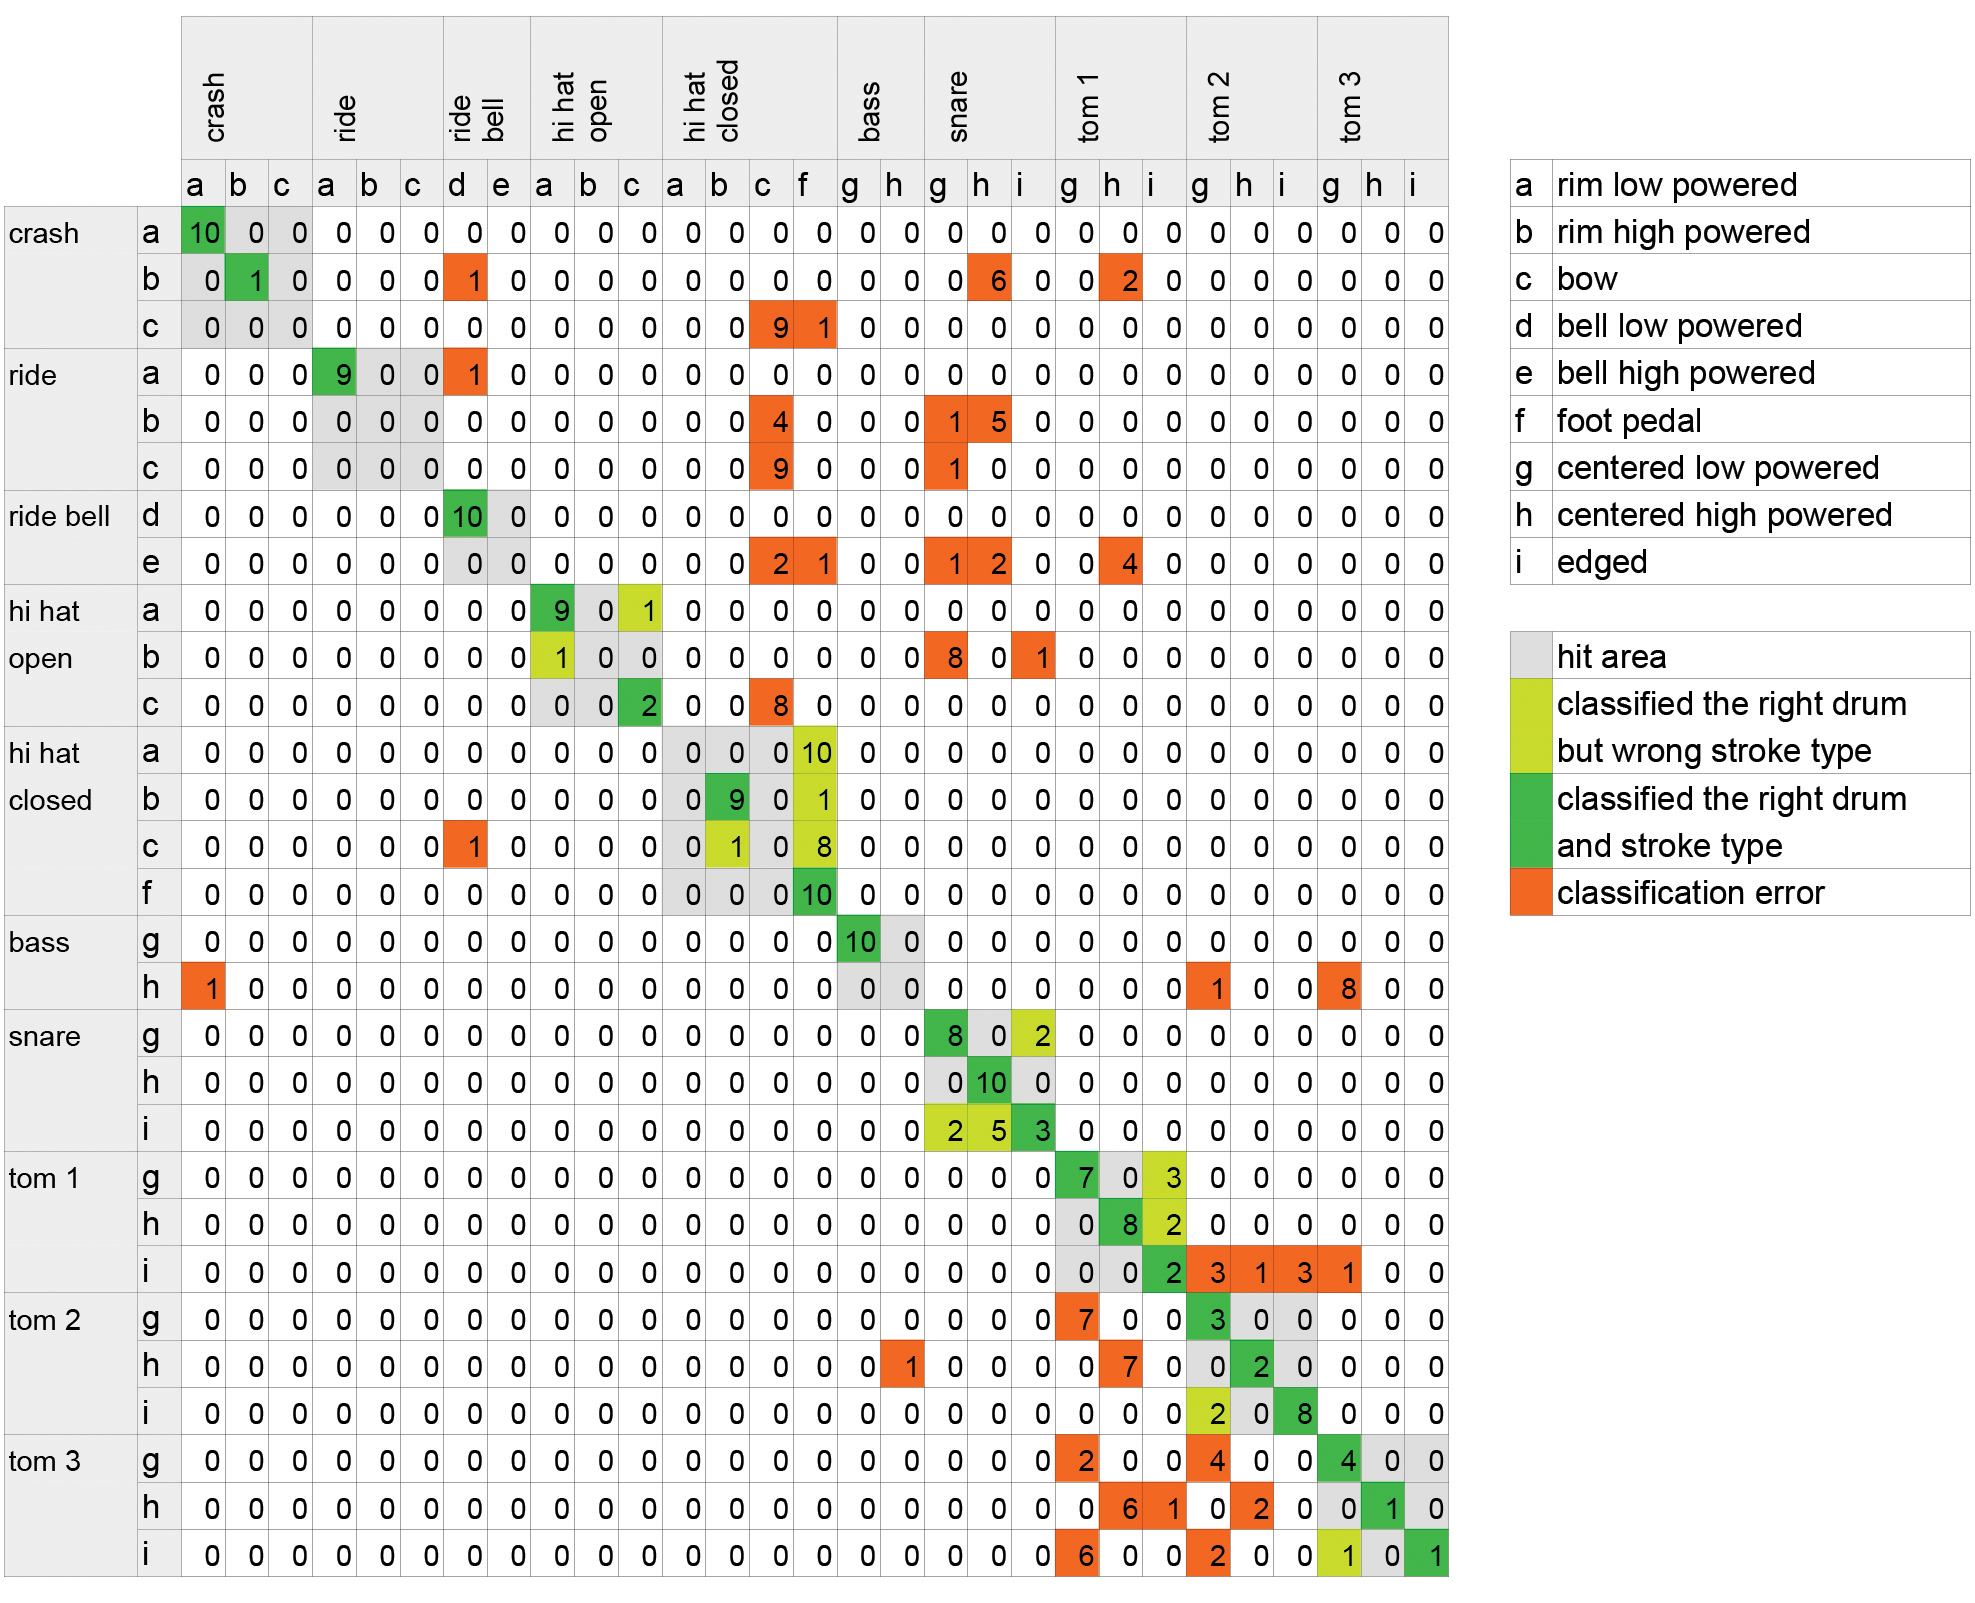
\includegraphics[width=\textwidth]{images/classification_matrix/matrix_test_1.png}
	\label{}
	\caption{Confusion matrix - method 1.}
	\label{fig:matrix1}
\end{figure}

The confusion matrix in figure (figure \ref{fig:matrix1}) shows the  result of this test. A hit-rate of 57.2 \% is reached for correctly classified drums and cymbals. Furthermore, 43.8 \% of the stroke types are identified.

The hit-rate for cymbals only is 48.0 \%. Here appear classification problems, especially for loud strokes and strokes on the rim. If only regular strokes (low to medium powered strokes), which are the most used ones by drummers, are considered, the hit-rate reaches 96.0 \%. Further on, the closed hi-hat, which is usually the most frequently played cymbal, only shows one classification error out of 40 tests.

For drums only are achieved more correctly classified instances than for the cymbals. The hit-rate reaches 60.0 \% here. But if only regular powered strokes are considered, the hit-rate merely reaches 74.0 \%, whereas the cymbals were classified correctly by 96.0 \%.

% länge von A variieren
 %betrachten unterschiedlicher frequenzbänder
 %bestes Ergebnis mit Frequenzband ....

\newpage
\subsubsection{Counting Frequency Bins in the Acceptable Range within a Predefined Frequency Band}
\label{section:shapeComparisonClassification2}

The second method for classifying drums and cymbals on basis of the minimum and maximum templates is developed by improving the preceding method.

Therefore, the distribution of frequency peaks in the frequency spectra of the different drums is considered. As described in section \ref{section:classificationSpectrumAnalysis}, the main peaks of the drums are located between 0 and 2000 Hz, whereas the cymbals show peaks in all frequency ranges. This fact leads to errors when comparing the entire frequency spectra to classify a drum because drums cannot be differentiated above 2000 Hz. Furthermore, the frequency peaks of the cymbals are more stable in a lower frequency band.

Hence, especially to improve the hit-rate for the drums, the comparison of the frequency bins with the templates is reduced to a frequency band from 0 to 2000 Hz. In a window of 2048 frequency bins for the entire spectrum, 2000 Hz are equivalent to 93 frequency bins. The other parts of the classification algorithm as well as  the pre-processing remains constant to the first method, which was described in section \ref{section:method1}. 

The result of the developed method is displayed in the confusion matrix in figure \ref{fig:matrix2}. As expected, the hit-rate for the classification of the drums is clearly improved. 80.7 \% is reached now, whereas only 60.0 \% were reached in the last test now. This is a rise of 20.7 \%. For regular strokes on drums only the hit-rate is improved by 12.0 \% from 74.0 \% to 86.0 \%. The hit-rate for the cymbals could even be improved more than the hit-rate of the drums. It rises by 43.3 \% from 48.0 \% to 91.3 \%. If only the regular strokes on cymbals are considered, the hit-rate  of 96.0 \% is the same as in the last test. The over all hit-rate is improved by 29.3 \% in relation to the preceding test from 57.2 \% to a hit-rate of 86.5 \%. Thereby, the stroke type is classified correctly with 63.1 \%. This is an improvement of 19.3 \%.

\begin{figure}[htb]
	\centering
	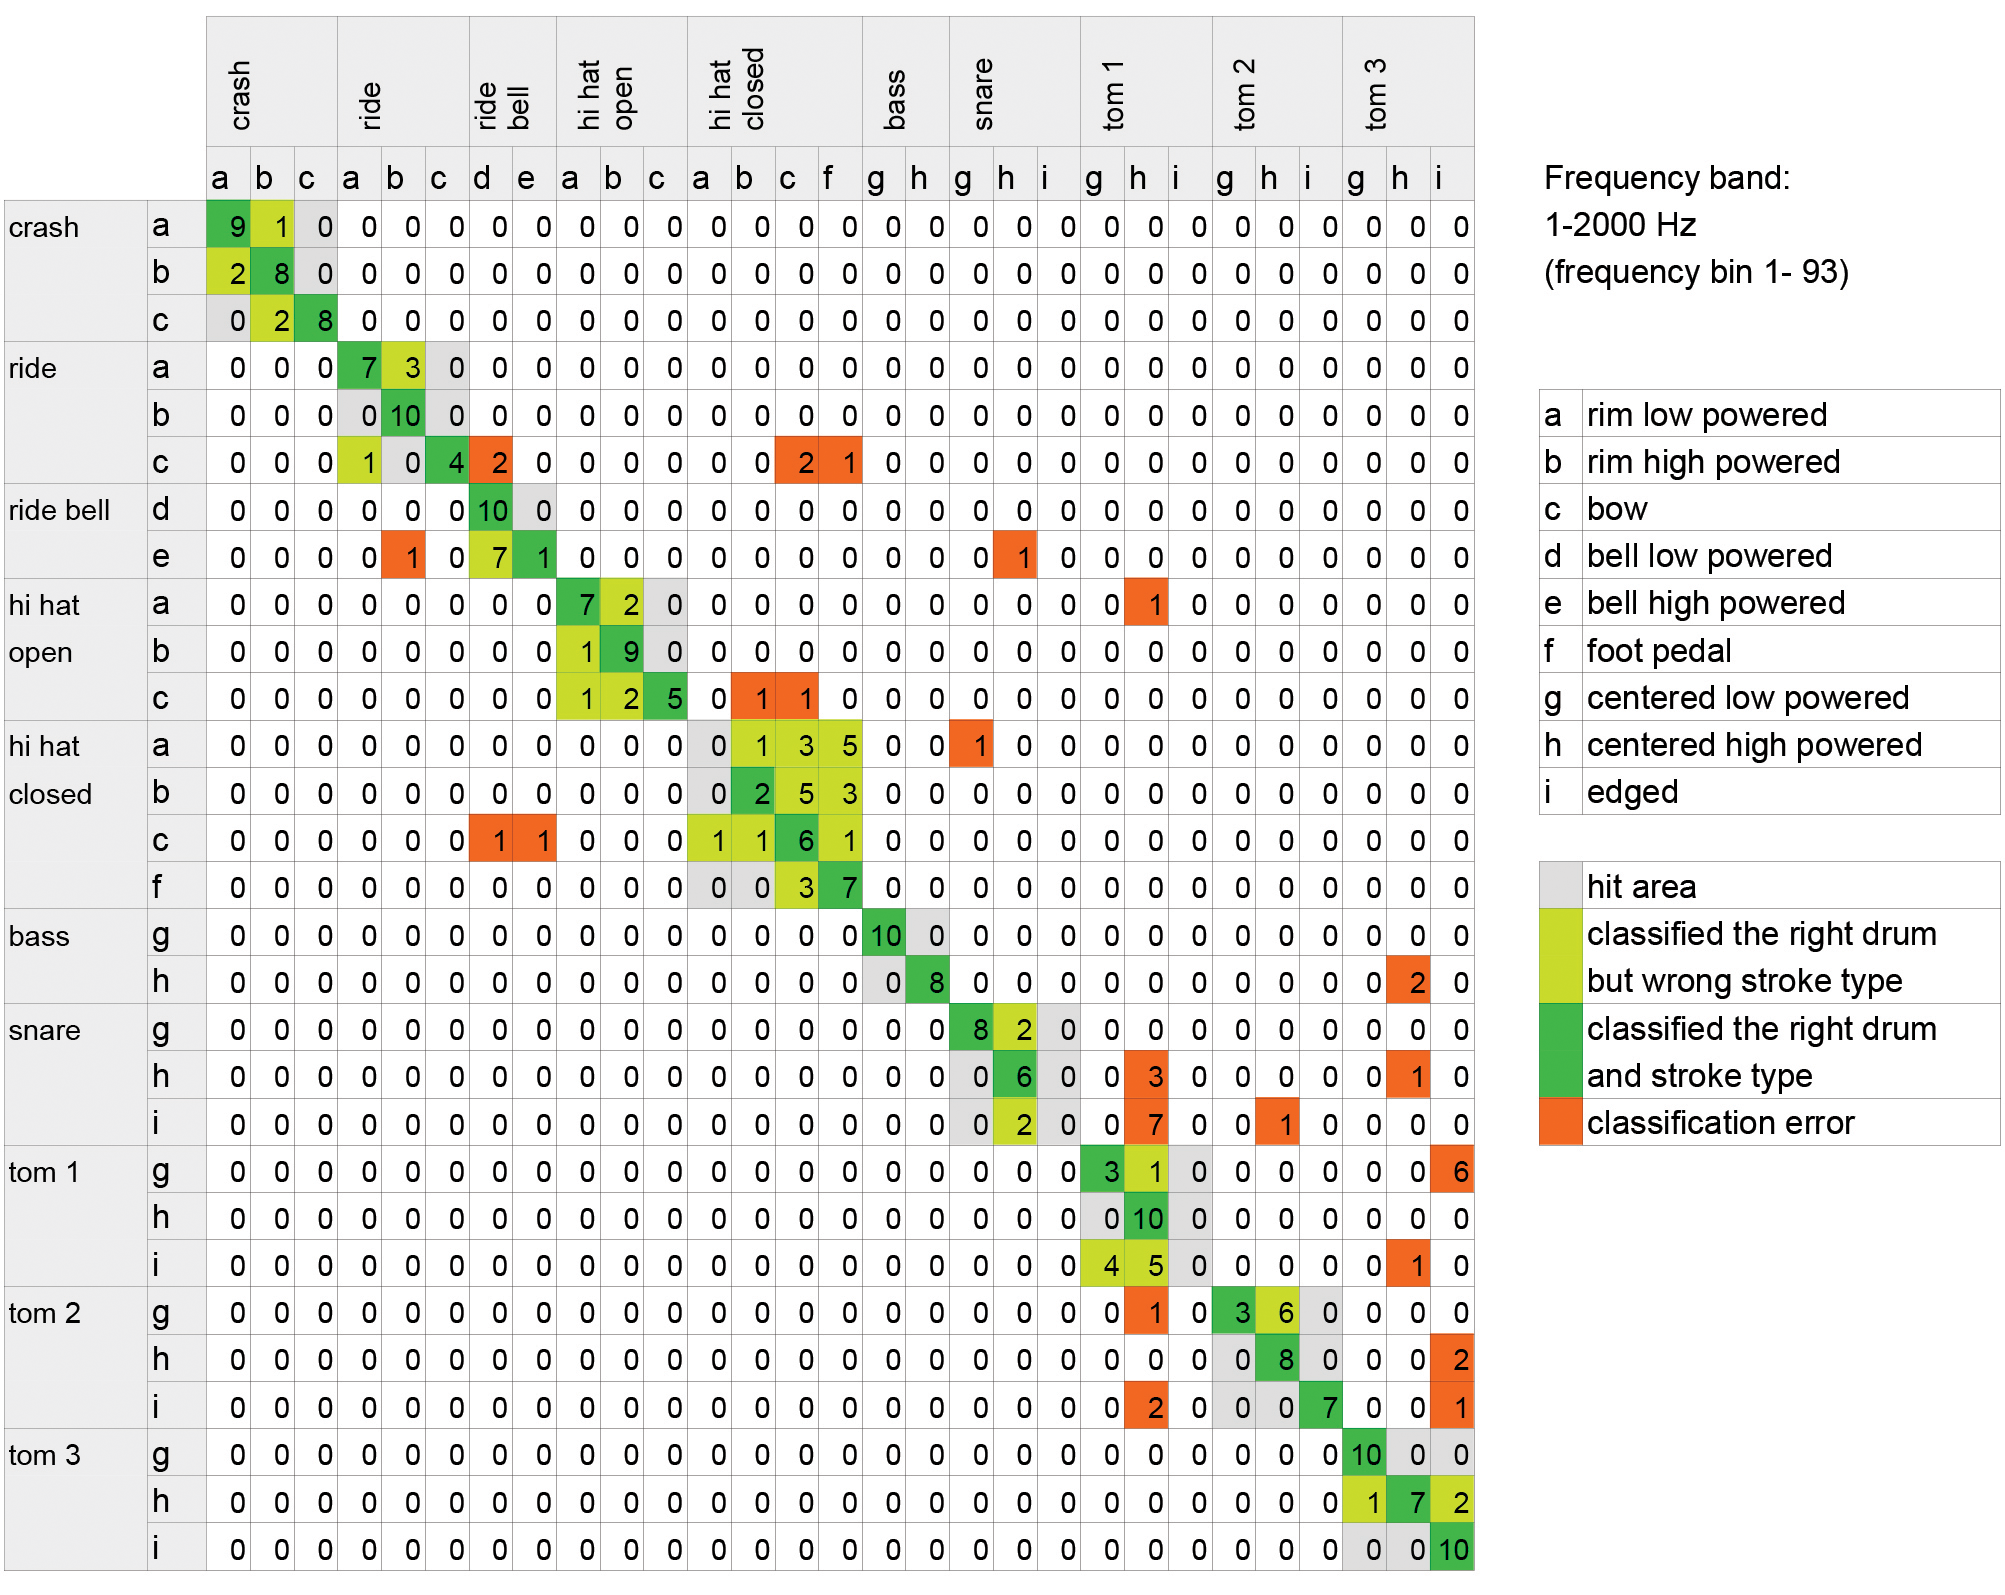
\includegraphics[width=\textwidth]{images/classification_matrix/matrix_test_2.png}
	\caption{Confusion matrix - method 2.}
	\label{fig:matrix2}
\end{figure}

%describe results of matrix 2
% gesamt 290
% hit 1 - 68
% hit 2 - 183 (63.1%)
% 1+ 2 = 251 (86.5%)
% miss - 39

%cymbals  (150)
% hit 1 - 45
% hit 2 - 92
% 1+2 = 137 (91.3 %)
% miss - 13
% regular strokes - 48/50 (96%)
% (ohne laute schläge und schläge auf bow)

%drums (140)  
% hit 1 - 23
% hit 2 - 90
% 1+2 = 113 (80.7%)
% miss - 32
% regular strokes - 43/50 (86%)
% (ohne laute schläge und schläge auf bow)


\newpage
\subsubsection{Calculating the Distance from the Acceptable Range}
\label{section:shapeComparisonClassification3}
%test quantile with distance from min/max

By classification method 3 the developed algorithm is improved again. The method is based on classification method 2, which was described in the preceding section. It focuses on the fact that there is only one stroke trained for each stroke type. This can cause errors in the preceding method because different strokes of the same stroke type can vary in their bin amplitudes. Thus, in some cases, the amplitude is not in the acceptable area, although the test stroke is compared with a matching template record. But in most cases the value is still close to the acceptable range. Usually, if the test record does not match the training record, the distance from the acceptable range is higher than the distance for non matching stroke types. Hence, the distance from the acceptable range is included in the algorithm. Instead of counting the bins outside the acceptable range as in the preceding approach, a simple distance function is applied. If a bin is placed outside the acceptable range, the distance of the bin to the area is added to the predefined distance variable \lstinline{distance}. The test instance is classified as the drum, where the template comparison returns the smallest distance value. The adapted MatLab\textsuperscript{\textregistered} code is shown in listing \ref{lst:testQuantileAD}.

\begin{lstlisting}[caption={testQuantileAD},label={lst:testQuantileAD}]
function[idxR]=testQuantileA(A,AMax,AMin)
	Results = zeros(1,length(AMax(:,1)));    
  for i = 1:length(AMax(:,1))
		distance = 0;  
		for j=1:372
			if A(j)<AMin(i,j)
				distance = distance + (AMin(i,j)-A(j));
      elseif A(j)>AMax(i,j)
				distance = distance + (A(j)-AMax(i,j));			
      end
		end
		Results(i) = distance; 
	end
	[minR,idxR]=min(Results);
end
\end{lstlisting}


For this approach, the best result is gained by considering a frequency band from 1 to 8000 Hz. For a 2048 bin window this matches the bins 1 to 372. The error rate for the drums that appeared in the first method is reduced due to the distance. The frequency bins for drums in a frequency range over 2000 Hz are all near zero. Thus, the distance to the acceptable area is approaching zero, too.

The resulting confusion matrix is displayed in figure \ref{fig:matrix3}. For the 290 test instances, there are only eight classification errors. This is a hit-rate of 97.2 \%, whereas 70.3 \% of the instances are classified with the correct stroke type. If only regular strokes are considered this method reaches a hit-rate of 100 \%. 

Furthermore, all drums are classified with the right class label, 84.3 \% of them even with the correct stroke type. The class labels for cymbals are classified correctly with 94.6 \%, whereby for 57.3 \% of them the right stroke type is determined as well.


%describe results of matrix 3
% gesamt 290
% hit 1 - 78
% hit 2 - 204 (70.3%)
% 1+ 2 = 282 (97.2%)
% miss - 8

%cymbals  (150)
% hit 1 - 56
% hit 2 - 86 (57.3%)
% 1+2 = 142 (94.6 %)
% miss - 8
% regular strokes - 50/50 (100%)
% (ohne laute schläge und schläge auf bow)

%drums (140)
% hit 1 - 22
% hit 2 - 118 (84.3%)
% 1+2 = 140 (100%)
% miss - 0
% regular strokes - 50/50 (100%)
% (ohne laute schläge und schläge auf bow)


\begin{figure}[htb]
	\centering
	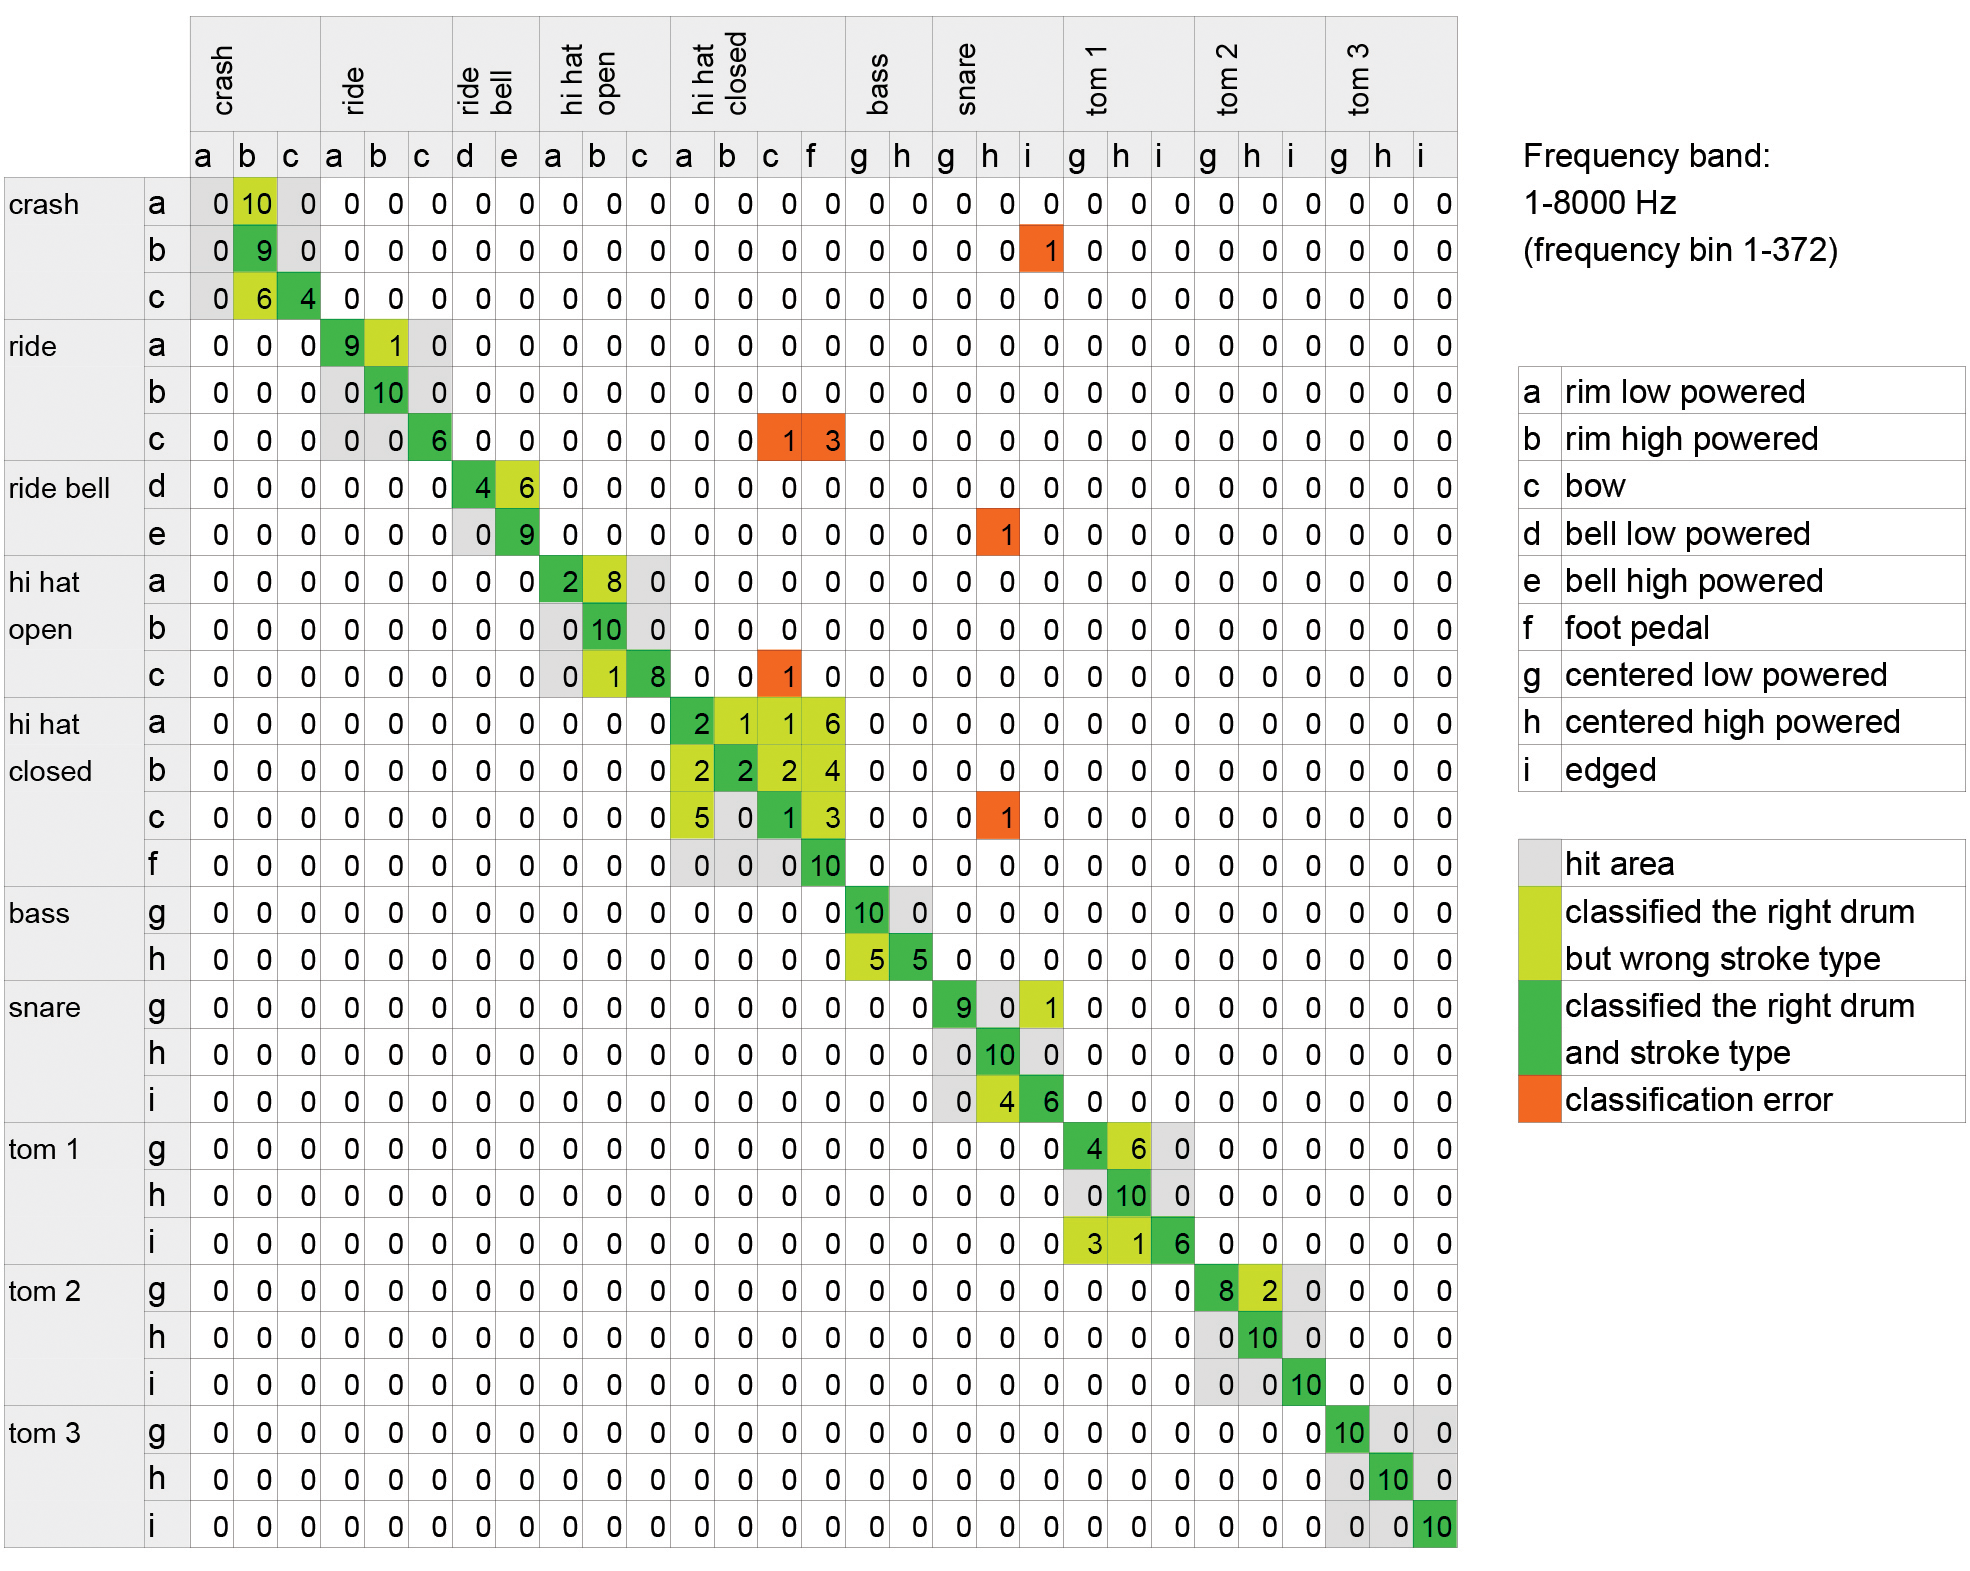
\includegraphics[width=\textwidth]{images/classification_matrix/matrix_test_3.png}
	\label{}
	\caption{Confusion matrix - method 3.}
	\label{fig:matrix3}
\end{figure}

%\newpage
%\subsubsection{The Use of Additional Features Using the Example Of the Steadiness}
%\label{section:shapeComparisonSteadiness}
%
%Next to the frequency spectrum, it is possible to use the approach described in the preceding with other features. An example feature which works with this approach is the steadiness, which was already used for the feature vector in the first classification method in section \ref{section:method1Features} of this thesis.

%test 4 quantile with distance from mean

%test 5 peaks

%Beim Testen passiert anschließend folgendes:
%Zunächst wird wieder ein Array mit 1024 Nullwerten erstellt und es werden die Peak Positionen des Testfiles gesucht.
%An jeder Position im Array, an der sich ein Peak befindet wird in der Trainingsmatrix der höchste Wert gesucht und im Array gespeichert. Dieser Wert repräsentiert die Drum, die am ehesten zu diesem Peak passt. 
%Nachdem alle Werte ins Array eingetragen sind werden diese gezählt. Der Wert, der am häufigsten vorkommt gewinnt. Als diese Drum wird das Testfile Klassifiziert.

%Result matrix:

%\subsubsection{Test results}



%%
	%\centering
	%\includegraphics[height=2cm]{images/templates12.jpg}
	%\label{}
	%\caption{Creation of templates for a minimum and maximum amplitude limit.}
	%\label{fig:templates12}
%\end{figure}]